\section{Bilder, Farbe, Perzeption}%
\label{bfp:sec:bilder_farbe_perzeption}

\subsection{Rasterbilder}%
\label{bfp:sub:rasterbilder}

Rasterbilder als hauptsächlicher Fokus (statt z.B Vektorgrafik)
\begin{itemize}
	\item Bild ist rechteckiges Pixelgitter endlicher Pixelzahl
	\item Digitaler \textbf{Framebuffer} als Kopie des Monitorbildes
	\item Pixel haben bestimmte \textbf{Farbtiefe}
	\begin{itemize}
		\item Schwarz/Weiß (1 Bit/Pixel), Graustufen (8 Bit/Pixel), True Color (24 Bit/Pixel)
		\item Farbe mit Farbtabelle (lookup table, \glqq LUT\grqq) und High Dynamic Range (3 x 32 Bit Floating Point/Pixel)
		\item Farbe wird i.d.R. durch RGB-Wert (Rot-Grün-Blau) charakterisiert
	\end{itemize}
\end{itemize}

\subsection{Bildtransfer zum Display}%
\label{bfp:sub:bildtransfer_zum_display}

Die Umsetzung eines digitalen Bildes zu einem sichtbaren Bild auf einem Display kann als \textbf{Transferfunktion f} betrachtet werden. Displaycharakteristika beeinflussen diese Darstellung, darunter:
\begin{itemize}
	\item Maximale Displayhelligkeit $I_{max}$
	\item Minimale Displayhelligkeit $I_{min}$ (Helligkeit eines schwarzen Pixels)
	\item Reflektiertes Umgebungslicht k
\end{itemize}
womit sich der erreichbare Kontrast $R_d = \frac{I_{max} + k}{I_{min} + k}$ ergibt. Man benötigt eine Transferfunktion, bei welcher der Unterschied zwischen aufeinanderfolgenden Pixelwerten nicht bemerkbar (unter 2\%) ist, um Color Banding zu vermeiden.

\subsection{Gamma-Korrektur}%
\label{bfp:sub:gamma_korrektur}

\textbf{Problem}:\\
Digitale Pixelwerte befinden sich in einem \textbf{linearen Raum}, d.h. doppelter Wert impliziert doppelte Helligkeit. Displays verhalten sich nicht linear, weshalb die Pixelwerte auf das Display angepasst werden müssen.
\\\\
Dieses Displayverhalten wird durch einen \textbf{Gamma-Wert} ($\gamma$) charakterisiert, die entsprechende Korrektur heißt \textbf{Gamma-Korrektur}. Die Intensität wächst nicht proportional zum Farbwert n bei N Schritten, sondern proportional zu $(\frac{n}{N})^{\gamma}$. Zur Gamma-Korrektur wird entsprechend jeder Farbkanal-Wert mit $\frac{1}{\gamma}$ potenziert.

\subsection{Alpha-Kanal}%
\label{bfp:sub:alpha_kanal}

Zusätzlich zu RGB-Farbwerten wird oftmals auch ein \textbf{Alpha-Kanal} gespeichert, dessen Inhalt die \textbf{Opazität} (Gegenteil von Transparenz) des Pixels ist.

\newpage
\subsection{Helligkeit}%
\label{bfp:sub:helligkeit}

\textbf{Weber-Fechner-Gesetz}\\
Subjektiv empfundene Stärke von Sinneseindrücken ist proportional zum Logarithmus der Intensität des
physikalischen Reizes.\\

Daraus ergibt sich eine kleiste wahrnehmbare Helligkeitsdifferenz $\Delta L_\text{JND}$
$$\frac{\Delta L_\text{JND}}{L} = \text{const} \approx 2\%$$
\begin{figure}[!h]
	\centering
    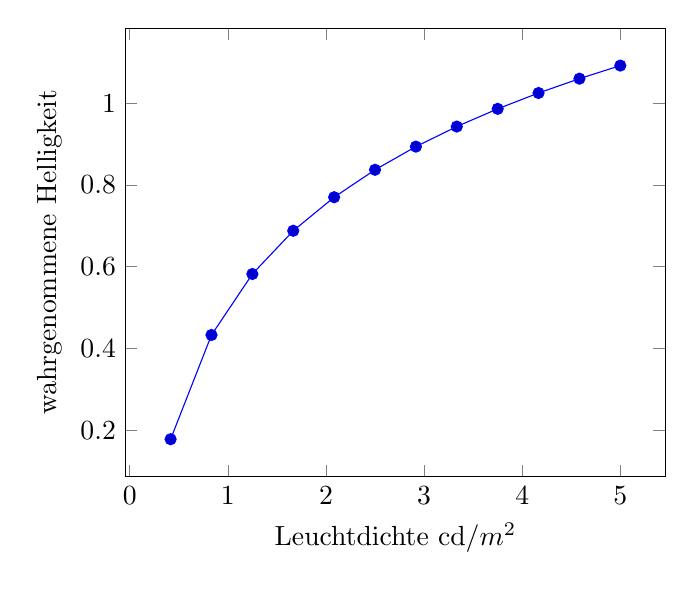
\begin{tikzpicture}
    	\begin{axis}[
    		xlabel=Leuchtdichte cd/$m^2$,
        	ylabel=wahrgenommene Helligkeit
        ]
        \addplot { 1 / e * ln x + 0.5};
        \end{axis}
    \end{tikzpicture}
\end{figure}
% TODO: Fix scaling of tikzpicture to go from 0 to 1 in both axes.

\subsection{Licht}%
\label{bfp:sub:licht}

\begin{itemize}
	\item Licht ist elektromagnetische Strahlung mit verschiedenen Charakteristika von Strahlen, Wellen und Teilchen
	\item Licht besitzt eine \textbf{Wellenlänge} $\lambda$, die u.a. eine Spektralfarbe repräsentiert\\(Lichtfrequenz $f = \frac{c}{\lambda}$)
	\item Sichtbares Licht: $380nm < \lambda < 780nm$
	\item Licht verschiedener Wellenlängen und verschiedener Intensitäten setzen weitere Farben zusammen
	\item \textbf{Metamerismus}: Unterschiedliche Spektren ergeben \textbf{dieselbe Farbe}
    \end{itemize}

\newpage
\subsection{Farbräume}%
\label{bfp:sub:farbraeume}

\textbf{Allgemein}:\\
Ein \textbf{Farbmodell} ermöglicht die Beschreibung von Farben durch Wertetupel, jedes Farbmodell erzeugt einen \textbf{Farbraum} aller möglichen Farben und diese können durch entsprechende \textbf{Tristimuluswerte} beschrieben werden.

\begin{itemize}
	\item Jeder Farbeindruck kann mit 3 Grundgrößen beschrieben werden (\textbf{Graßmannsche Gesetze})
	\item \textbf{Additive Farbmischung} (vgl. RGB-Farbmodell)
	\begin{itemize}
		\item Summe der Tristimuluswerte Rot, Grün und Blau ergibt finalen Farbwert
	\end{itemize}
	\item \textbf{Subtraktive Farbmischung} (vgl. CMY(K)-Farbmodell)
	\begin{itemize}
		\item Statt RGB: Cyan, Magenta, Yellow (und in der Praxis Schwarz als 4. Key-Color, da CMY typischerweise kein Schwarz ergibt)
		\item Differenz der Farbwerte ergibt finalen Farbwert
	\end{itemize}
	\item \textbf{Weder additiv noch subtraktiv} (vgl. HSV-Farbmodell)
	\begin{itemize}
		\item Charakterisierung der finalen Farbe durch Farbton (Hue), Sättigung (Saturation) und Helligkeit (Value)
	\end{itemize}
\end{itemize}

\subsection{Farbraumkonversion}%
\label{bfp:sub:farbraumkonversion}

\textbf{Ziel}: Farbraum zur standardisierten Konversion zwischen Farbräumen.\\\\
\textbf{Color Matching Funktionen}
	\begin{itemize}
		\item Reproduktion von Spektralfarben durch RGB-Primärfarben
		\item RGB ist kein perfekter Farbraum, manche Spektralfarben sind nicht realisierbar!
	\end{itemize}		
\textbf{XYZ-Farbraum}
	\begin{itemize}
		\item Beschreibt alle wahrnehmbaren Farben (\glqq Gamut der menschlichen Wahrnehmung\grqq) mit rein positiven Color Matching Funktionen
		\item Primärfarben sind imaginär, übersaturiert und nicht physikalisch realisierbar
		\item Lineare Abbildung $XYZ \Leftrightarrow RGB$, Transformationsmatrix $M$
		\item Problem: $M^{-1}$ enthält negative Werte, XYZ kann auf negative, nicht darstellbare RGB Werte abbilden
	\end{itemize}
\textbf{xyY-Farbraum}
	\begin{itemize}
		\item \textbf{Beobachtung}: $kX, kY, kZ (k > 0)$ repräsentiert dieselbe Farbe mit unterschiedlicher Intensität
		\item \textbf{Idee}: Normalisierung auf der $X + Y + Z = 1$ Ebene, daraufhin Projektion auf die XY-Ebene (z weglassen)
		\item \textbf{Ergebnis}: Weiterhin alle Farbtöne und -sättigungen in XY erhalten, neuer xyY Farbraum mit Helligkeit Y und Farbe/Chromatizität xy
	\end{itemize}